\documentclass[11pt, xcolor=dvipsnames]{article}
\usepackage{graphicx}
\usepackage[colorlinks=true,citecolor=red,urlcolor=blue]{hyperref}
\usepackage{geometry}
 \geometry{
 a4paper,
 total={170mm,240mm},
 left=20mm,
 top=25mm,
 }


% \title{STC Project Proposal \\ Analysis of magnetic field oscillation in adiabatic slower}

% \author{Yu Lu id Dept. of Physics\\ Xingyao Wang id Dept. of \\ Nitish Mittal id Dept. of}
% \date{\today}

\begin{document}
\begingroup  
  \centering
  \LARGE STC Project Report\\[0.5em]
  \large Yu Lu (id:yl25684) \\  Nitish Mittal (id:nm23456)\\Xingyao Wang (id:xw2695)\\[0.5em]\par
  \large Github \url{https://github.com/SuperYuLu/STC-2016} \\ [5mm]
  \large Dec. 12, 2016\\
  \endgroup
  
%\maketitle
\section{Introduction}
Adiabatic slower is a facility that consist of hundreds of overlapping Anti-Helmholtz coils, which is used to slow atoms from $\sim 500 m/s$ down to $\sim 0 m/s$ to create ultra bright cold atom source in atomic physics. It is realized by activiting apatially overlapped magnetic traps with a overlapping time sequence, thus create an effective co-moving trap to slow down atoms. While its performance has been highly evaluated in the experiment\footnote{E. Narevicious, et. al., New Journal of Physics 13 (2011)}, the optimization hasn't been well discussed in any published articles. One of the key feature is the magnetic field oscillation during the trasition of traps, which is related to the lose rate, temperature, density of atoms being slowed. Here we propose a simulation approach to this problem. As a first order approach, we will simulate the transition of magnetic field with a constant speed. we will discuss the oscillation of magnetic field in adiabatic slower under different conditions, such as current pulse shape, time sequence, geometry setup, etc. The program is been realized in C++, python3, Makefield and Shell  command.

\section{Description of purpose}
Anti-Helmholtz coil is a pair of coils with current in it propogating at opposite direction. Some atoms at special quantum states tend to stay at the magnetic field minimum to lower their energy, as shown in figure \ref{fig1}, where only the field along atom moving axis is shown, while the trap itself is a 3D trap, which is the reson atoms can be trapped at the minimum point of field.\\ \begin{figure}[h]\centering  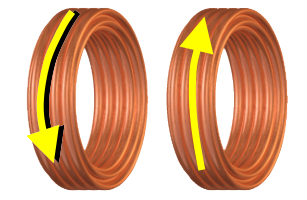
\includegraphics[width = 0.2\textwidth, height= 0.15\textwidth]{antiHelmholtz} 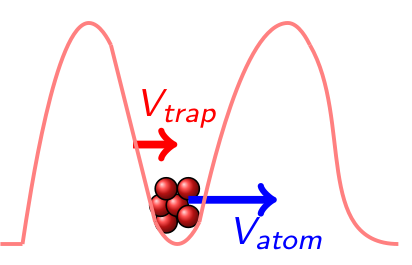
\includegraphics[width = 0.2\textwidth, height= 0.15\textwidth]{trap} \caption{(A) Anti-Helmholtz coil. (B) Atoms in the magnetic trap} \label{fig1} \end{figure} The trap basically provide a confinement of atoms, and can be treated as a 'carrier'. If we can control the moving speed of this 'carrier', then we can control the atoms confined by it. To realize this, a series of this kind of traps are activated in an overlapping sequence, both in real space and in time space, thus an effective moving trap can be created, as shown in \ref{fig2}. Usually these traps are switched on and off with hundreds of microseconds.\\\begin{figure}[h!]\centering 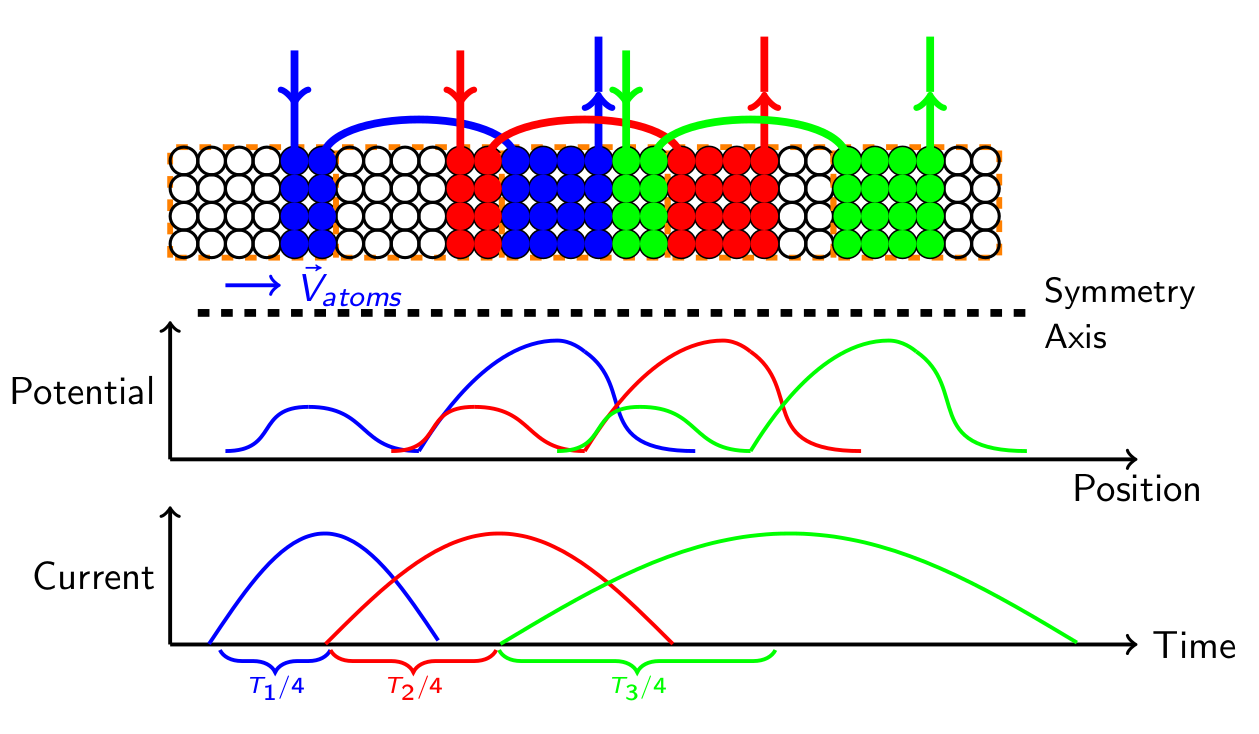
\includegraphics[width = 0.5\textwidth, height=0.3\textwidth]{switching} \caption{Schematic for generating co-moving magnetic trap} \label{fig2}\end{figure}

Since it is not possible to realize a smoothly moving magnetic field with speed of about $500 m/s$ in the real world, one has to consider the possible discontinus when the total filed is transfered from one Anti-Helmholtz coil pair to another. As shown in figure \ref{fig2}, the crossection view show that different coil pairs(same color for same pair) are spatially overlapped by some amount of distance, the current in the coil basically decides when the specific coil should be switched on and off. Due to the overlapped geometry and timing sequence, the field generated by these coils are also overlapped.\\

One can obviouse see that the magnetic field transistion will be depend on the geometry, the current pulse length and shape, and also the switching speed. On this project we are trying to study:\begin{itemize} \item  Magnetic field transition with different current pulse shape: sine and trangle shape. \item Magnetic field transition with different overlapping of geometry and current sequence.\item The oscillation of Magnetic field minimum under different conditions as above.\end{itemize}

\section{Program structure}
The main part of this project is based on C++ object-oriented programming, to make debug and optimization easier, makefile combined with python3 and shell command were used. Here is a brief review of how the simulation is been realized. \\
\subsection{C++ program}
Our C++ program is used to generate simulation data, save it in the $/dat$ directory. These data will be used by Python3 program to generate plots.\\

\textbf{main.cc} Define an 1D array of class ''\textit{traps}'', the dimension of the array is decided by the total number of traps we are simulating. Based on given global varialbles in the header file, calculate the total length of the traps and the total time and steps to do the simulation. After the 1D array of class were created, loop through them to give each trap a specific number, and based this trap number call the mathod of this class to initiate the position of each trap, together with their ''turn on'' time. Then according to presetted simulation time step, loop through the simulaiton ''\textit{clock}'' by incressing one step eatch time.  For each spacific time, loop through all of the traps, for each trap call a certain method to calculate the magnetic field within and neighboring the coil pair. After this is done for a specific time, the magnetic field generated by each of the traps should already been calculated and stored in of the objects for the class. Since we are interested in the total field rather than the field generate by a specific single coil, then we call a function to calculate the total field by direct adding the field value with the same posistion and same time. This total field will be saved in the directory $/dat$ as .CSV with time (in microseconds) as the name of the file. By the end of running the programming, the total field at different time should be saved in different files to be used later by the python program. \\

\textbf{traps.h} Define the class \textit{''traps''}, it has objects: trapNum(for trap number), tStart(the turn on time), tEnd(the turn off time), zStart(the calculation starting position), clock(store the simulation clock), centerPos (the center position of trap), frontCoil(the position of front coil) and backCoil(the position of back coil). Also it has method: initTrap(initialize trap parameters based on the given trap number), isOn(Check if the trap is turned on), calCurrent( calculate current value at specific time), calField(based calculated current, calculate the Magnetic field at specific position), genFieldMatrix( genrate the field value matrix, with position and field value as matrix elements) and cleanField(clear stored value by last simulation step)\\

\textbf{initTrap} Function,initialize the trap geometry based on the trap number.\\

\textbf{isOn.cc} Function, based on the clock and the specific traps number, calculate if a specific trap should be ''turned on''. \\

\textbf{calCurrent.cc} Function, calculate the current based on the current shape and clock.\\

\textbf{calField.cc} Function, calculate the Magnetic field at specific position and time\\

\textbf{genFieldMatrix.cc} Function, generate the field through our a region by specific trap, save it in an array for later use.\\

\textbf{calTotalField.cc} Function, add the field up for the same position and time.\\

\textbf{findFieldMin.cc} Find the field minimum of the total field, give it's value and position.\\

\textbf{csvWriteAll.cc} Function, write the total field at specific time in to a .CSV file.\\

\textbf{csvWriteMin.cc} Function, like above, but only save the filed minimum information in a .CSV file. \\

\textbf{main.h} Include all the declarition of functions and libraries used by the main program.\\

\textbf{const.h} Include all the global variables, and simulation settings, act as the control pannel.\\

\subsection{Python3 program}
Since one cannot use C/C++ to generate nice plots, here we wrote a python3 script to do the plotting. The python3 code basically automatically look into the $/dat$ directory, automatically distinguish the file name and do the plot of field distribution. Another similar python3 program is used to plot the position and velocity of Magnetic field minimum.\\

\subsection{Shell script}
To be better review the simulation result, one want to make animation of the field with the changing time. To do this, a open source softerware \textit{ImageMagick} has been used and called. It is set to conver all of the plots generate by our python3 program into a .gif animation, it also written to automatically detect the file name so that the animation sequence will not be massed up.

\subsection{MakeFile}
Since we have so many seperate .cc files and diffrent codes to run, it is better combine all of them into a MakeFile. In the makefile, it does the complie work for C++ to generate the executable, at the same time, it has also embeded with ability to call python3 code and shell script, additionally, some phony commands have also been written into makefile to clean up the directry, creat tar ball of the surce code.

\section{Running the program}
Here is a brief Introduction how to run the simulation:\begin{enumerate} \item Modify the global variables in const.h file to control the simulation parameters \item run ''\textit{make}'' the generate .o and executable files \item run ''\textit{make plotall}'' to call python3 to plot all field distributions. \item run ''\textit{make plotmin}'' to plot the infomation of the field minimum \item run ''\textit{make gif}'' generate the gif animation file. \item run ''\textit{clear}'' to remove all of the .CSV data files \item run ''\textit{clean}'' to remove executable and .o files \end{enumerate}
\section{Result and Discussion}
Based on our program, we discussed about the field dependence on the current pulse shape, timing sequence and geometry. The basics settings are, according to experiment real situation: \begin{description} \item[Coil radius]: 5mm  \item[Coil pair space] 10 mm \item [Coil overlap distance] 5mm  \item[Simulation space step] 0.05 mm/step \item[Current pulse period] 50 us \item[Simulation time step] 0.5 us \item[Coil windings] 16 \item[Total trap numbers] 5 \end{description}

\subsection{Magnetic field at different time}
Since we have about 70 figures showing how the magnetic build up and decrease with time, here I only picked a few just to give a sence how it looks like, as shown in figure \ref{fig3}.
\begin{figure}[h] \label{fig3} \centering 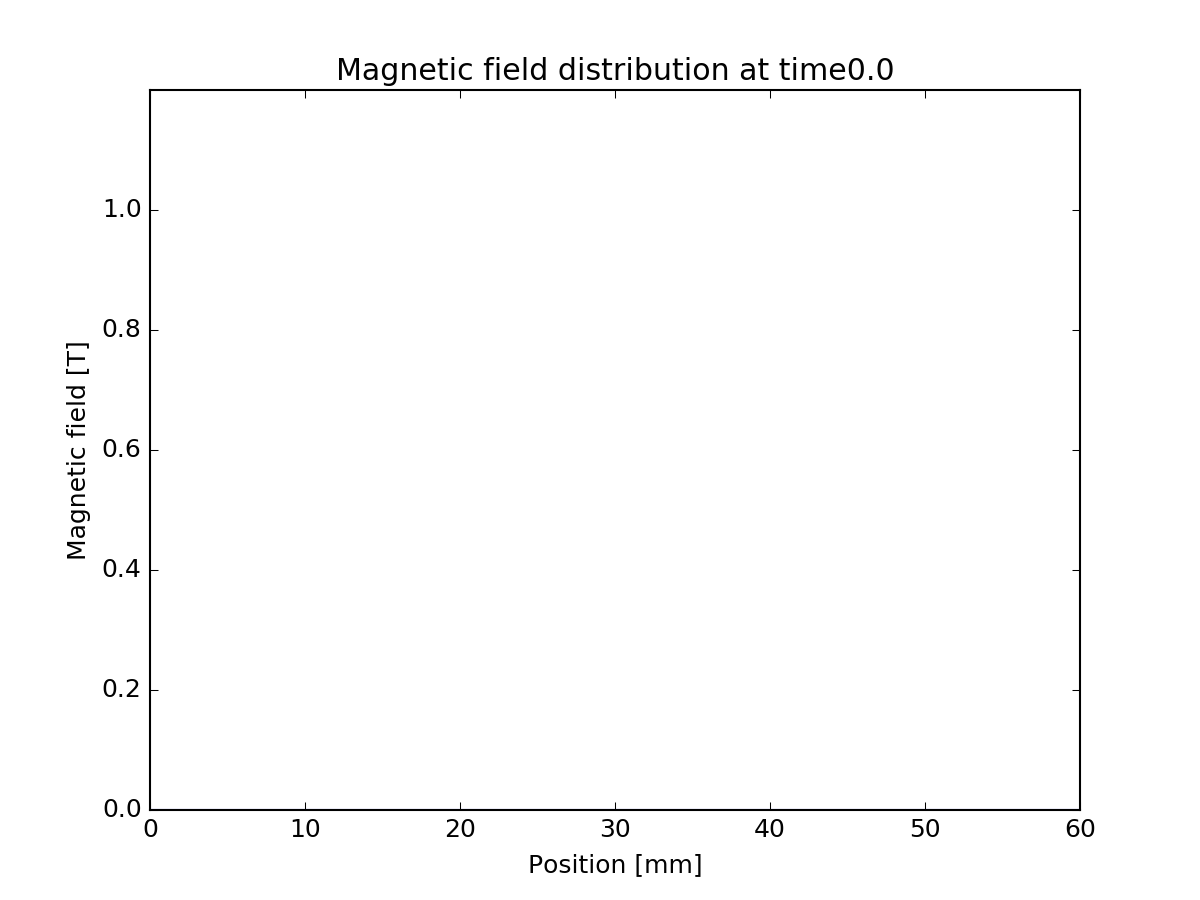
\includegraphics[width = 0.4\textwidth]{00.png} 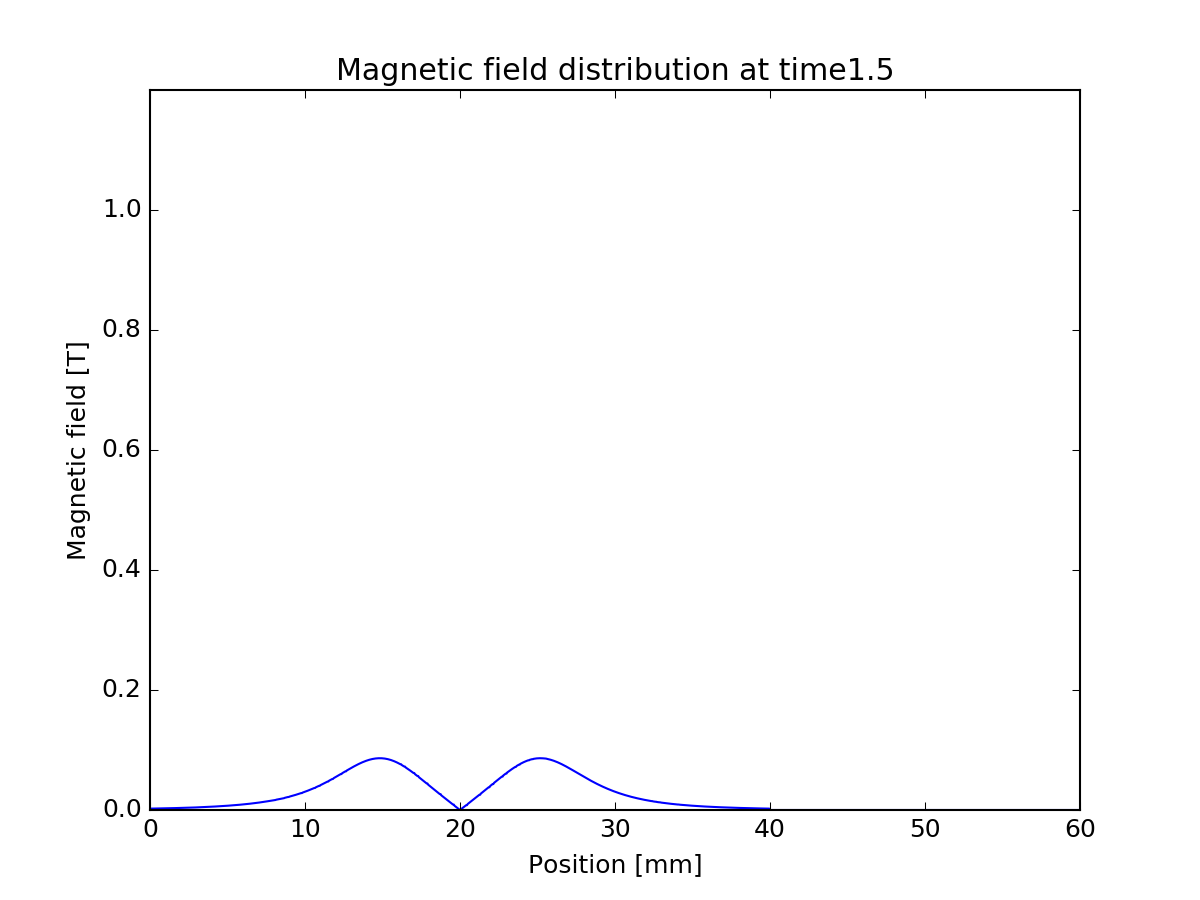
\includegraphics[width = 0.4\textwidth]{15.png}\\ 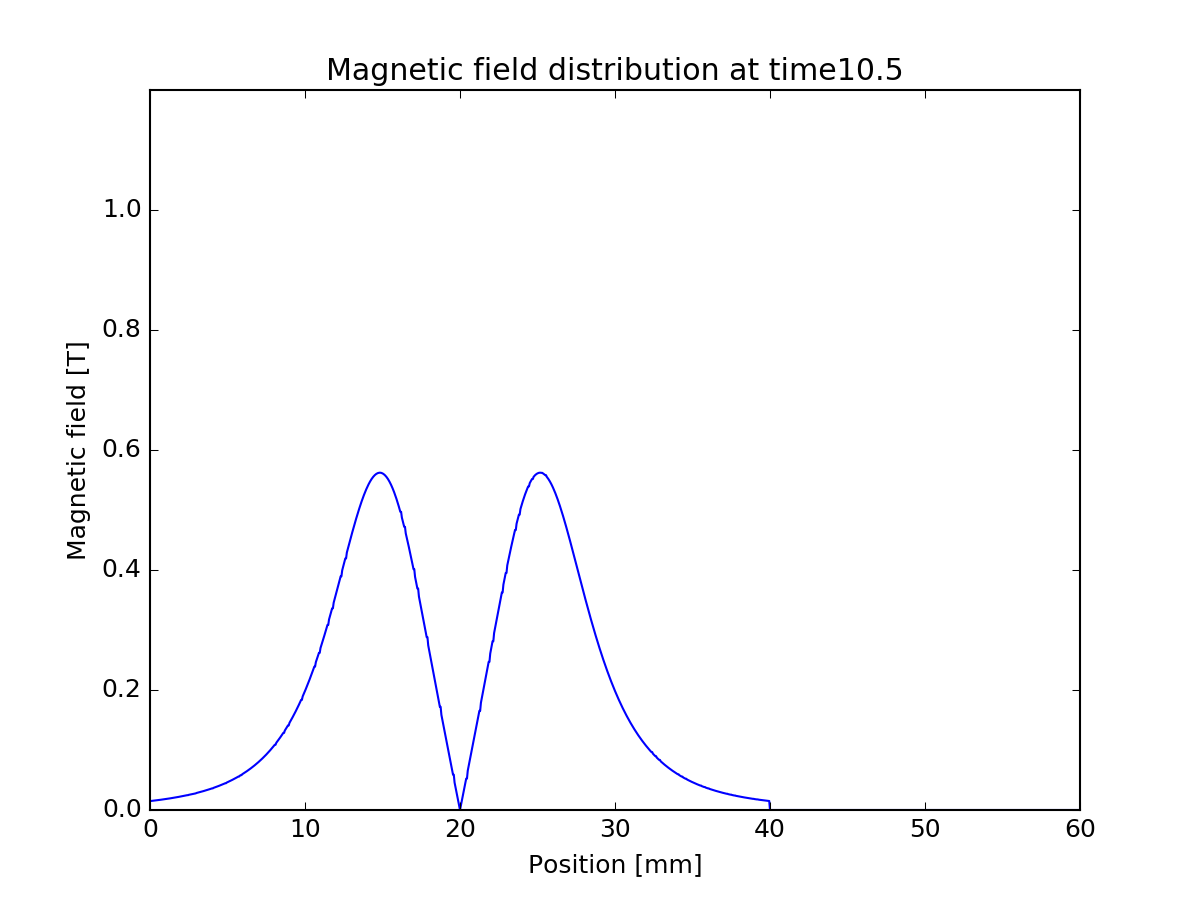
\includegraphics[width = 0.4\textwidth]{105.png} 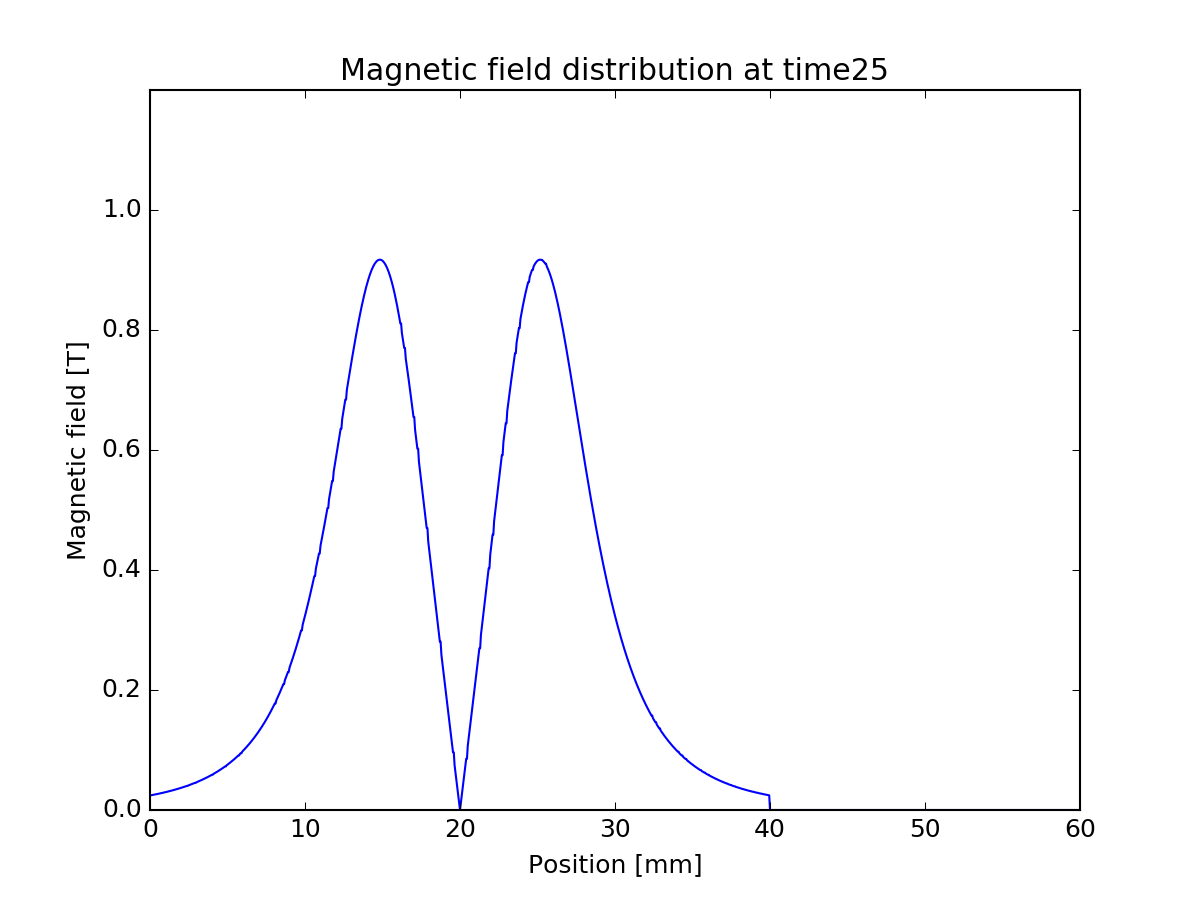
\includegraphics[width = 0.4\textwidth]{25.png} 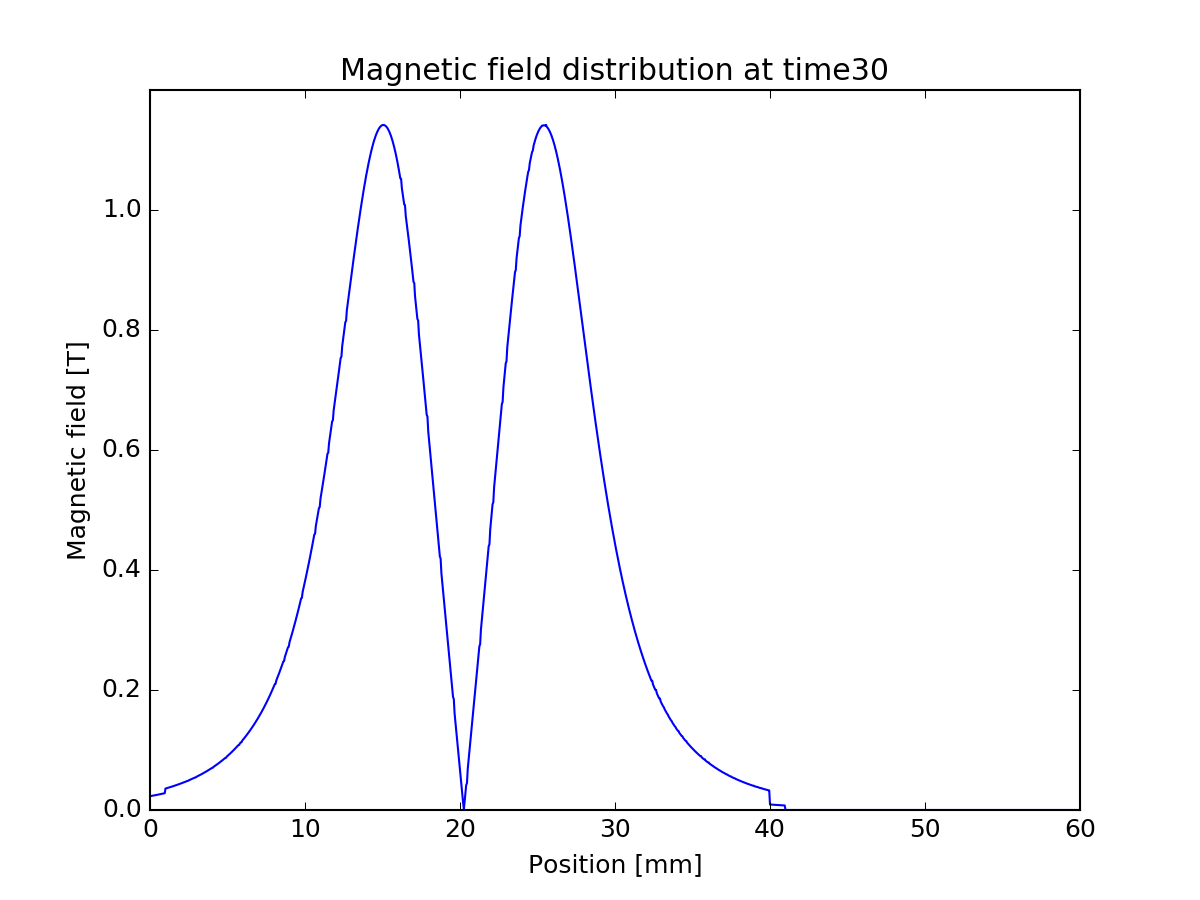
\includegraphics[width = 0.4\textwidth]{30.png} 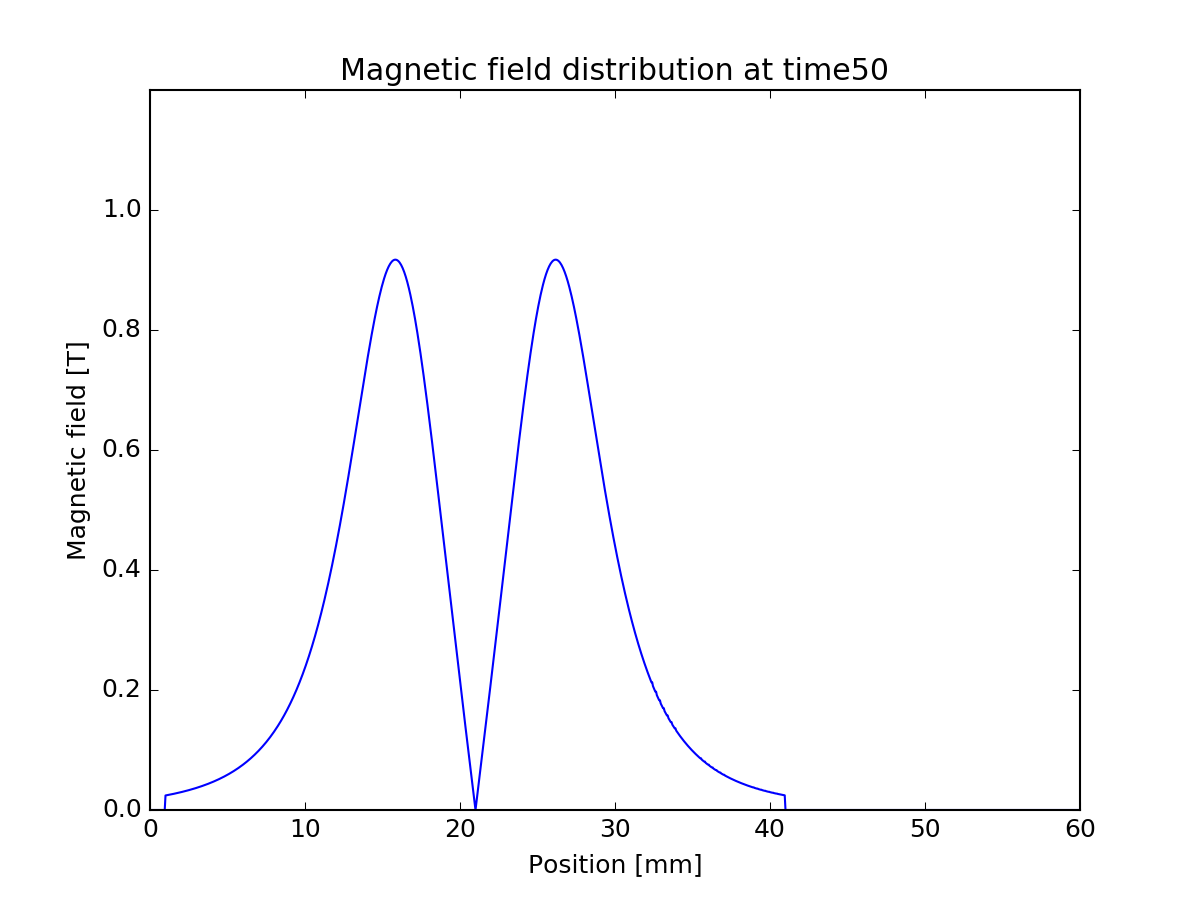
\includegraphics[width = 0.4\textwidth]{50.png} \caption{Magnetic field at different times. title of each figure give the time in microseconds}\end{figure}

\subsection{Magnetic field oscillation --- Sine and Triangle current}
Based on the general settings, we varied the current pulse shape. We used the sine wave and triangle wave current signal, trying to study field minimum positoin, velocity, minimum value. As shown in figure \ref{fig4}  \begin{figure}[h] \centering \label{fig4} 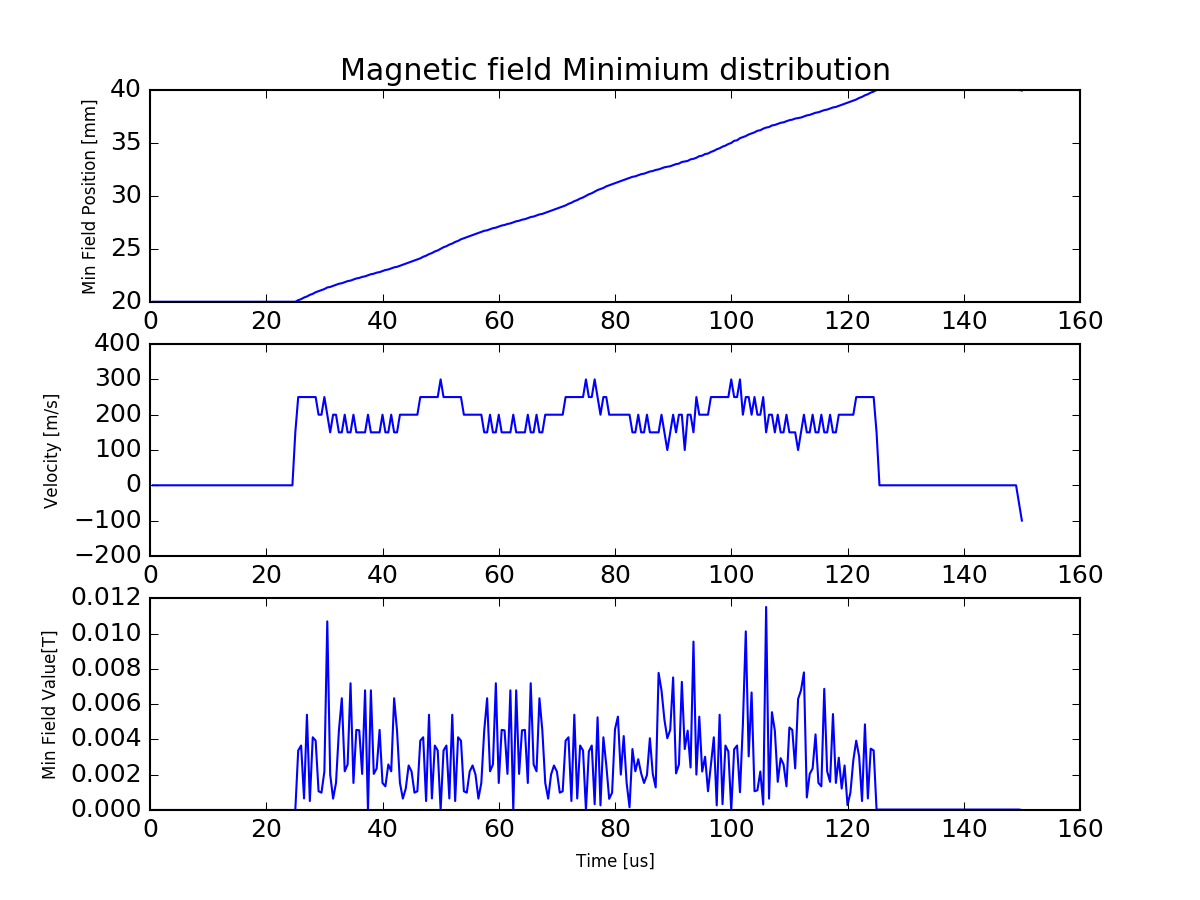
\includegraphics[width = 0.49\textwidth]{sine_toverlap_5} 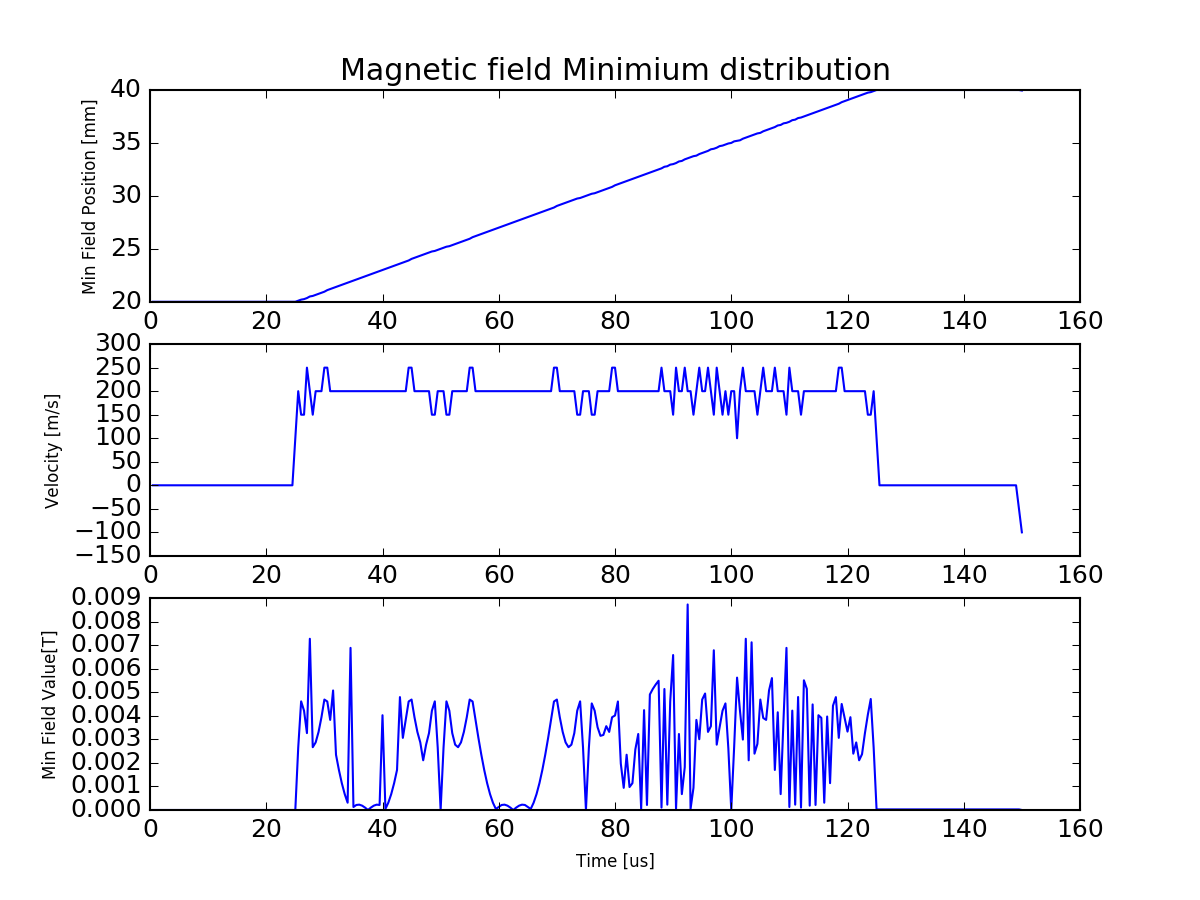
\includegraphics[width = 0.49\textwidth]{triangle_toverlap_5} \caption{Magnetic field minimum position, velocity and field value, under different current pulse conditions: (a)Sine wave current pulse; (b)Triangle wave current pulse} \end{figure} 
\\
\textbf{Discussion} From figure \ref{fig4}, compare the two plots of the field minimum distribution, one can see that: \begin{itemize} \item The Magnetic field minimum generally traverls with a averagely constant velocity during the transition. \item Based on our setting, the velocity is oscillating with a small range. \item The actually value of field minimum is not always 0 (ideal situation), but oscillating with some small value. \item since shape current has higher average transition velocity compare to the triangle shaped current pulse. \item Triangle shaped current pulse has relatively lower oscillation.  \end{itemize}


\subsection{Geometry overlap effects}
In addtion to the current pulse, we alse discussed the trap geometry overlap distance, as shown figure \ref{fig5} \\ \begin{figure}[!t] \label{fig5} 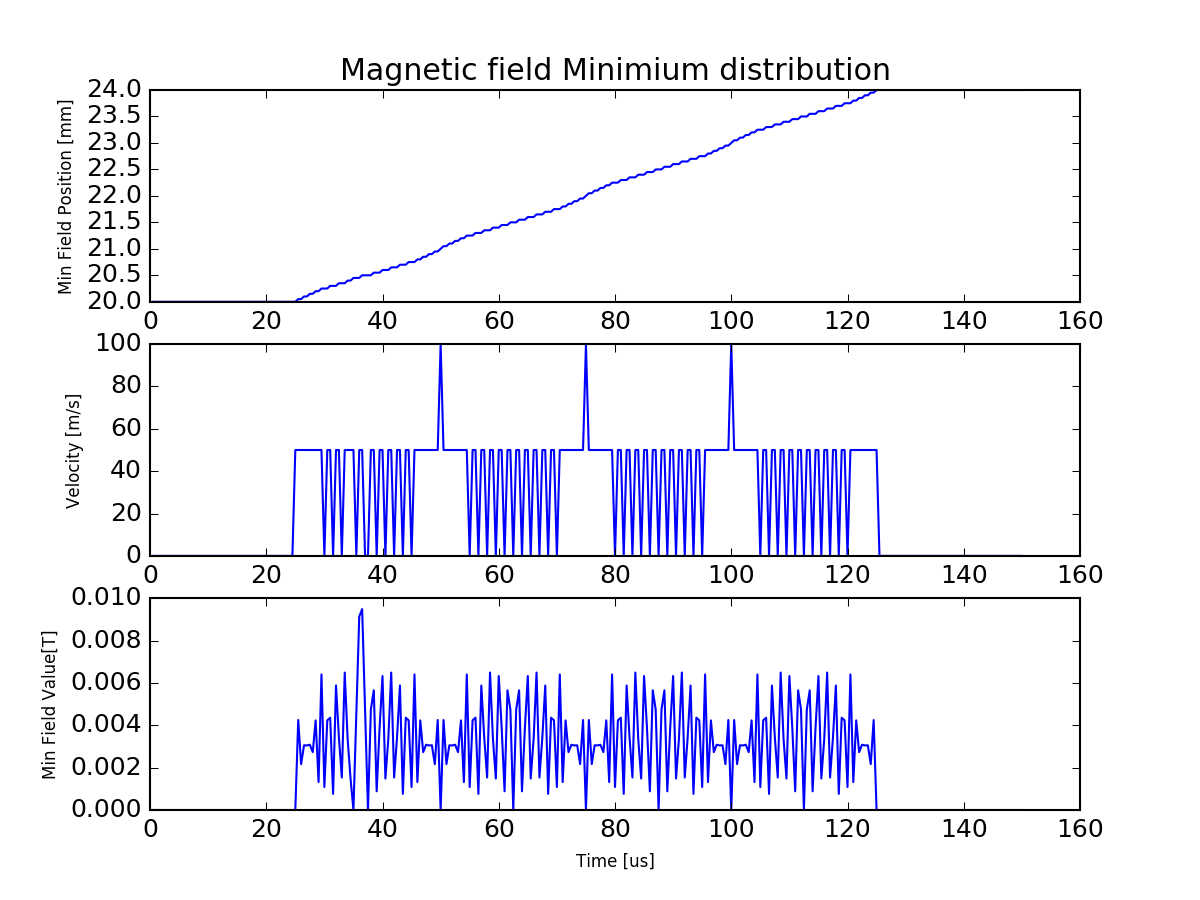
\includegraphics[width=0.45\textwidth]{sine_goverlap_3}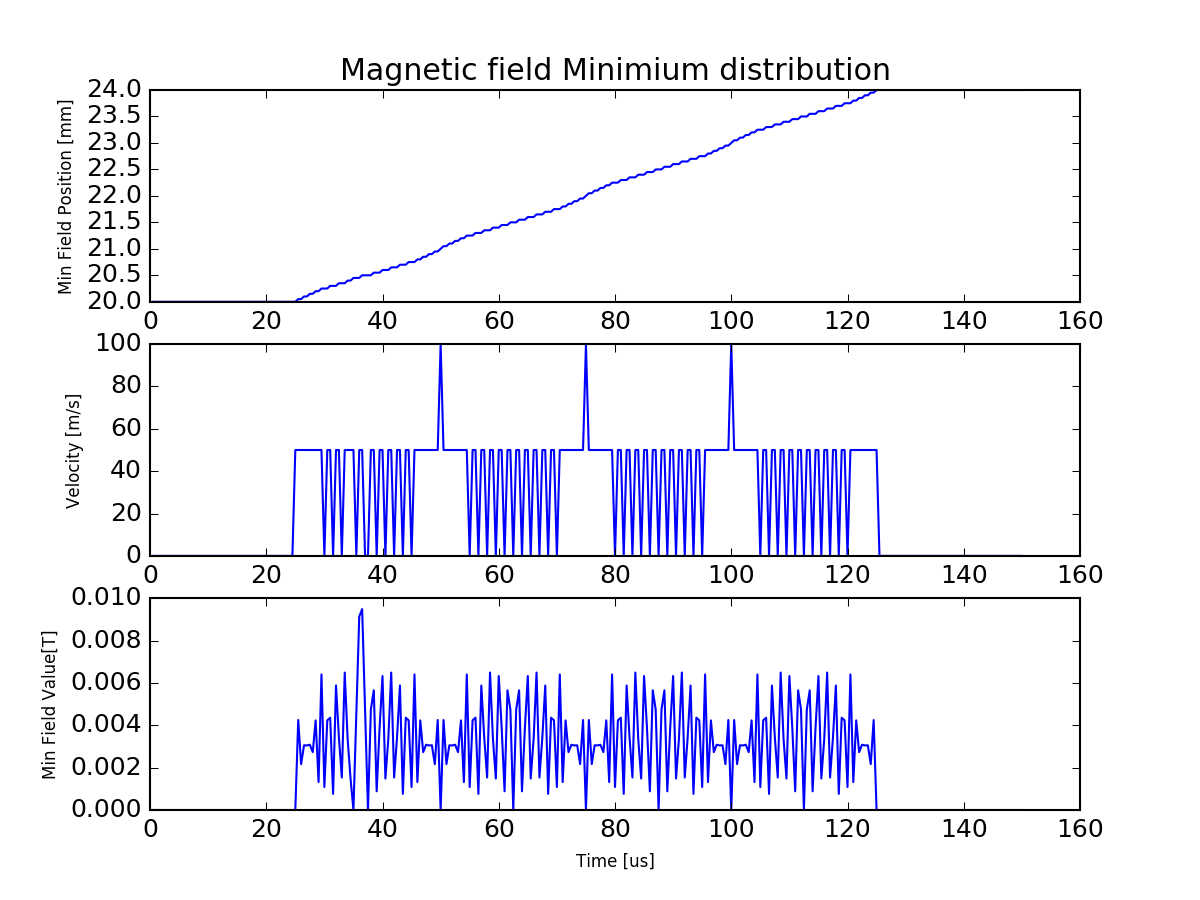
\includegraphics[width=0.45\textwidth]{sine_goverlap_4} \\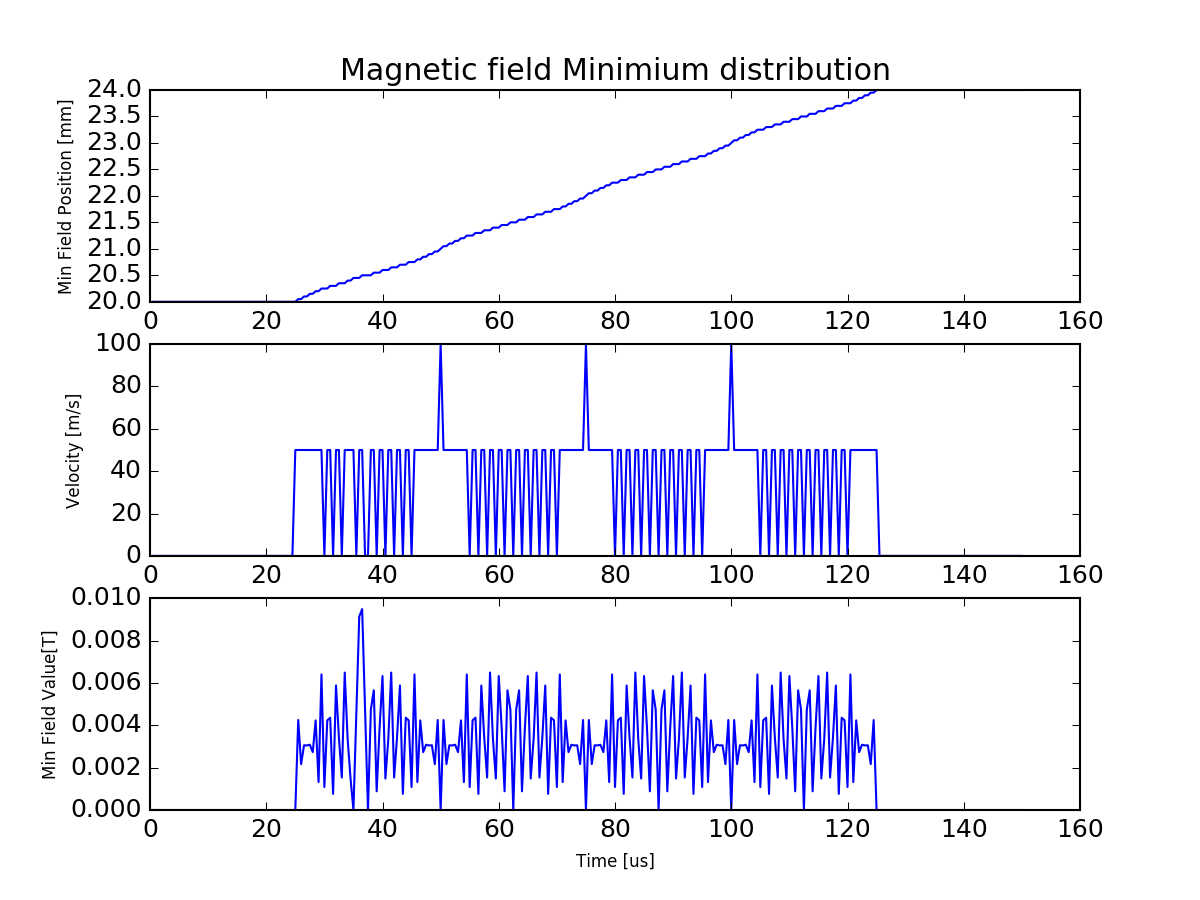
\includegraphics[width=0.45\textwidth]{sine_goverlap_5}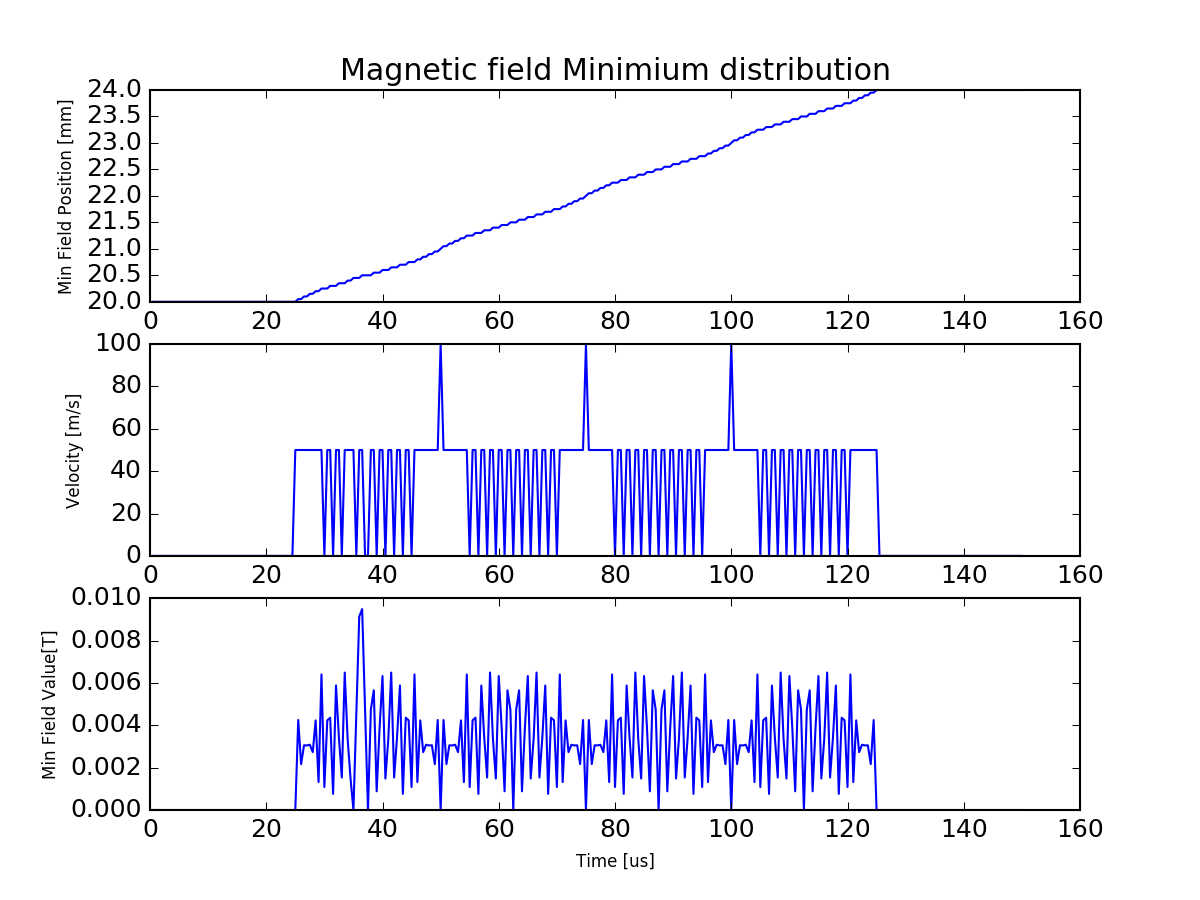
\includegraphics[width=0.45\textwidth]{sine_goverlap_6}\\ 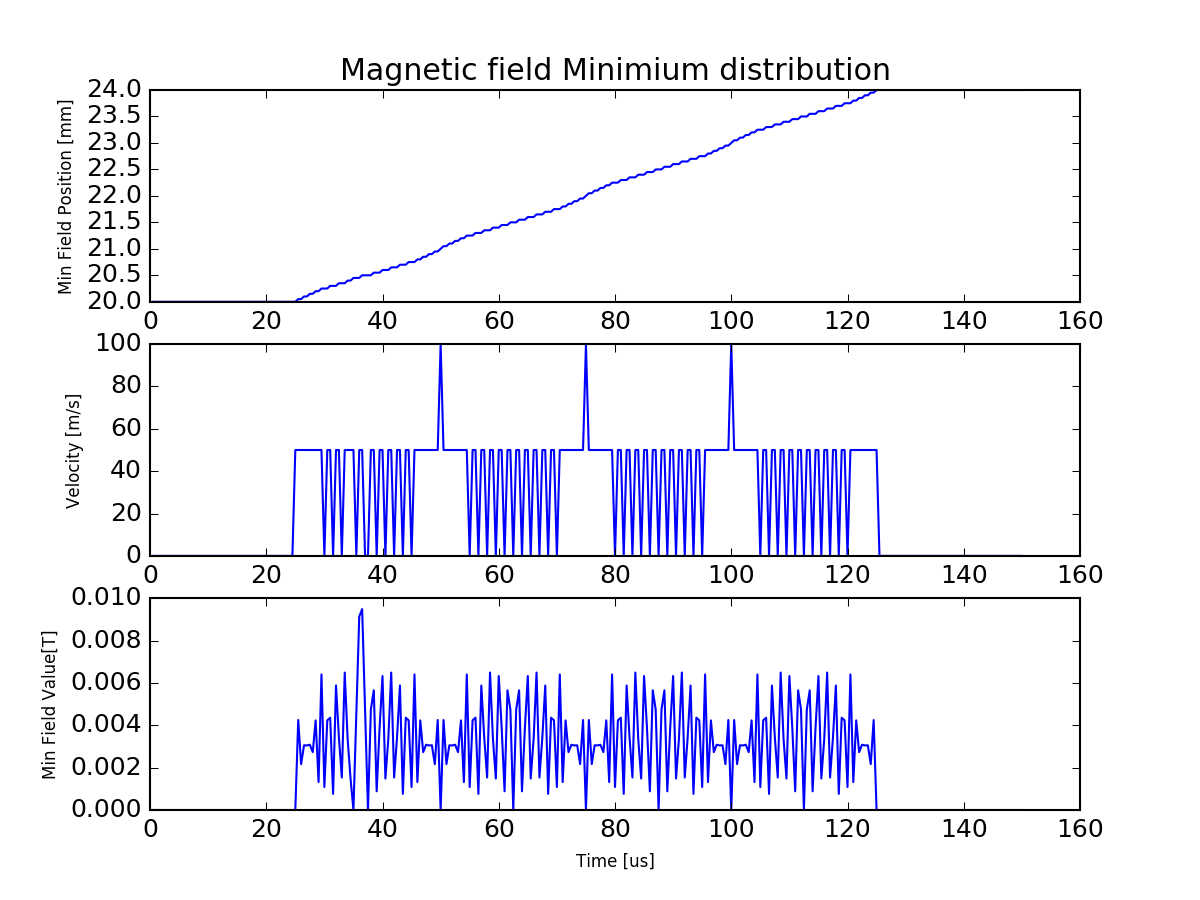
\includegraphics[width=0.45\textwidth]{sine_goverlap_7}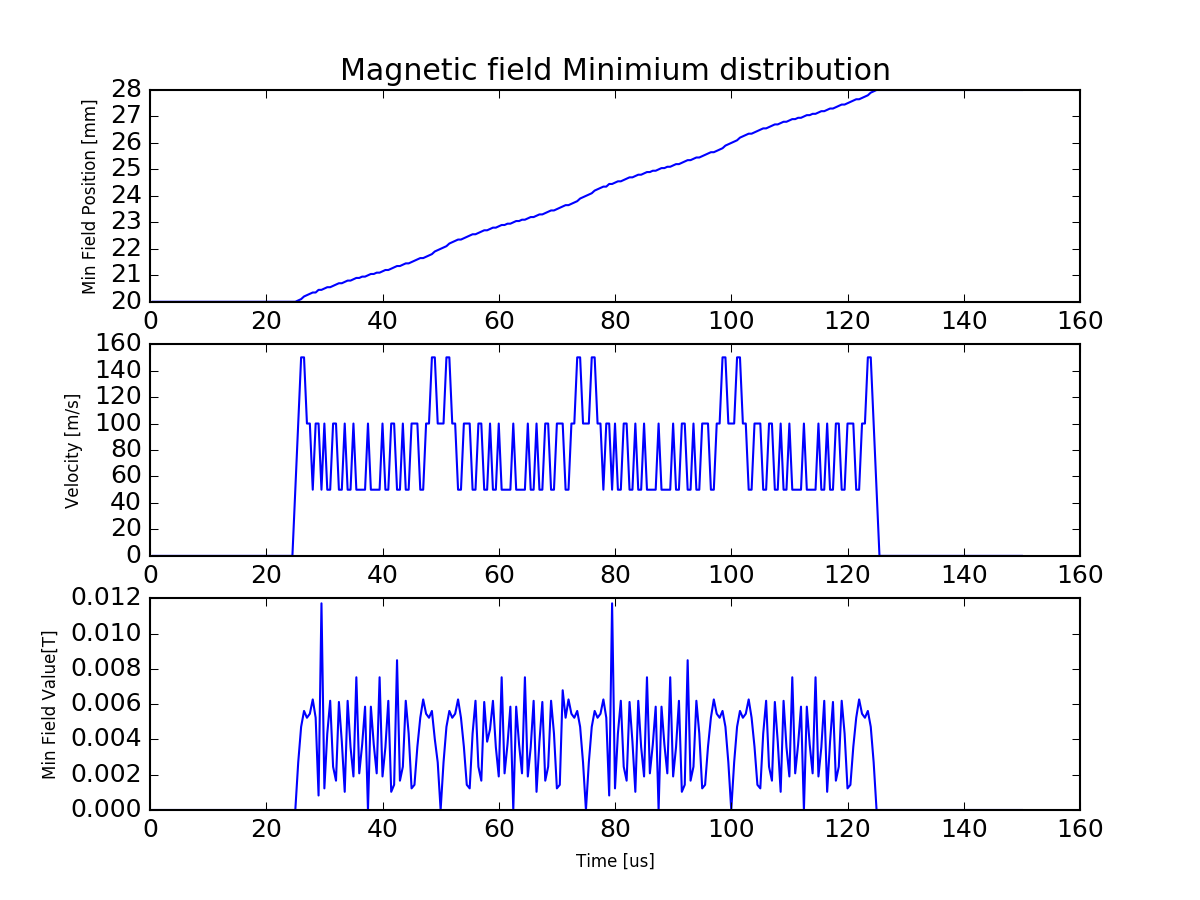
\includegraphics[width=0.45\textwidth]{sine_goverlap_8} \caption{Magnetic field oscillation under different trap coil Geometry overlap: (a)Overlap 3mm;(b)Overlap 4mm;(c)Overlap 5mm;(d)Overlap 6mm;(e)Overlap 7mm;(f)Overlap 8mm.} \end{figure}
\textbf{Discussion} From the different Geometry Overlapping, one can see the oscillation of the minimum field is always there. When the Overlapping distance range from 3 mm to 8 mm, the speed of transition doesn't change to much except when the overlapping is too long, such as 8 mm. So the conclusion is that the field minimium oscillation is not sensity on the geometry overlap distance, which mean in the lab it does not matter if one make some mistake of the Overlapping distance by a short length.

\subsection{Time overlap effects}
As the same with the Geometry Overlapp effects, we also discussed the time overlap effects, by varying the current push overlap time, as shown in figure \ref{fig6} \\ \begin{figure}[!t] \label{fig6} 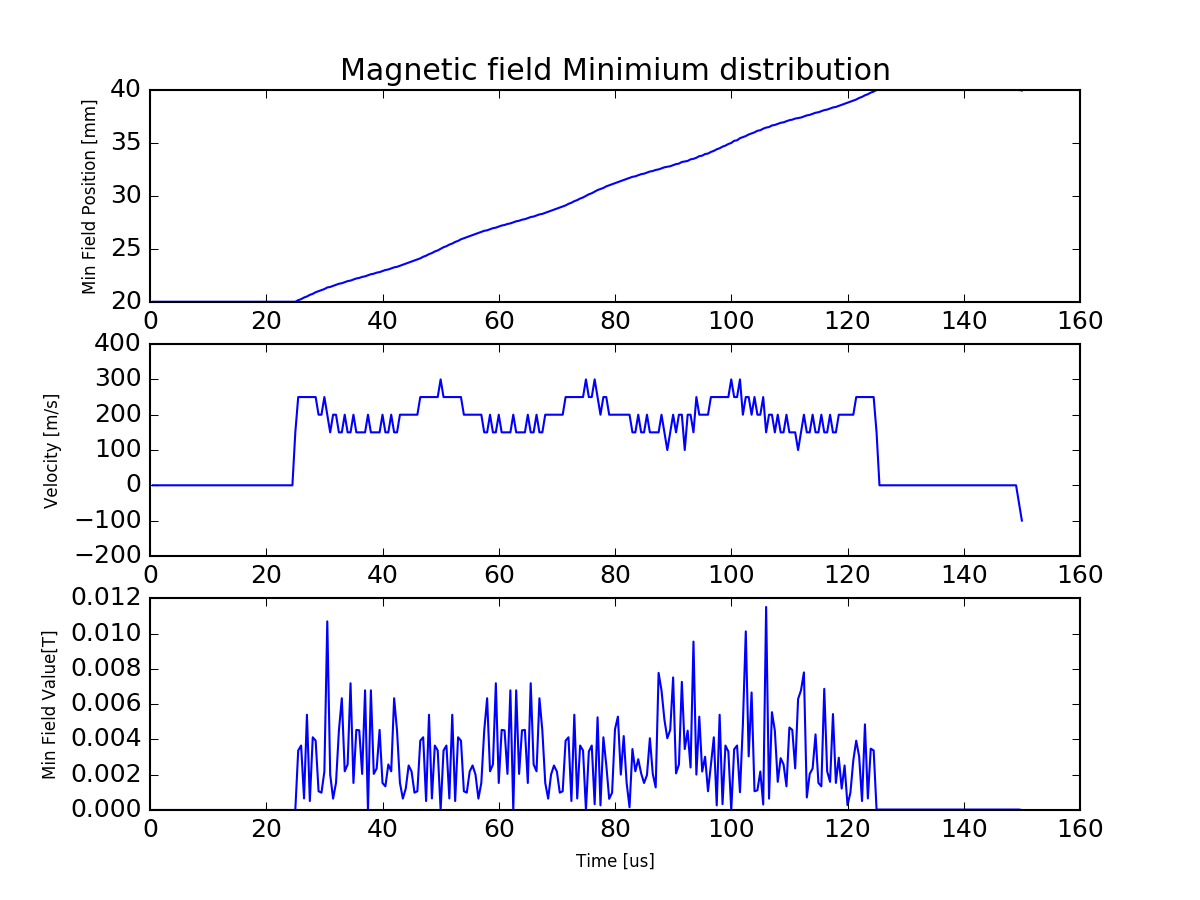
\includegraphics[width = 0.45\textwidth]{sine_toverlap_5} 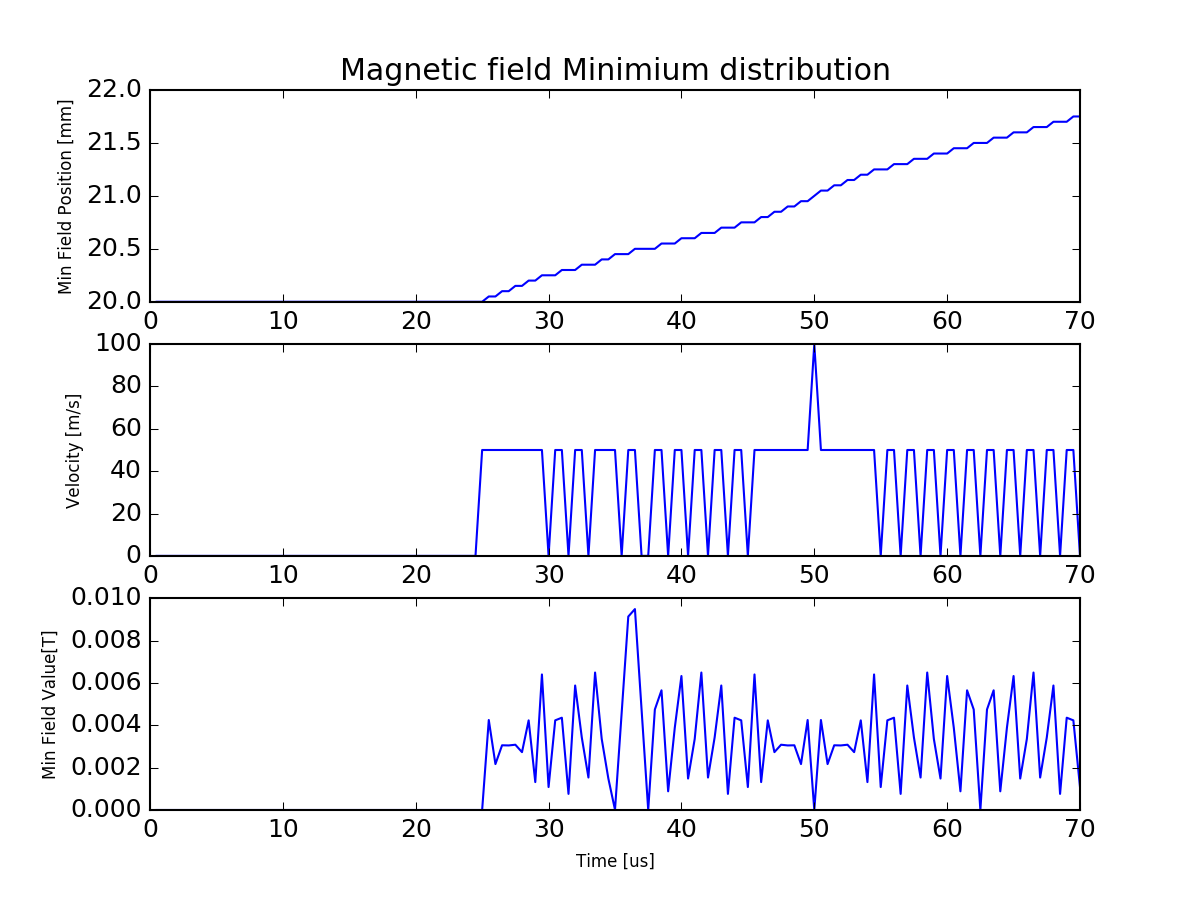
\includegraphics[width = 0.45\textwidth]{sine_toverlap_9} \caption{Magnetic field oscillation under different current pulse Overlap: (a) Time overlap 25 us (b) Time overlap 45us} \end{figure}
\textbf{Discussion} From the two plot, one can see that the longer time Overlapping reduces the average speed a lot. Interms of the minimum field oscillation, the longer Overlapping pulse length has a relatively lower oscillation frequency, but the oscillation amplitude is about the same, compare the the shorter time Overlapping.

\section{Summary}
In this project, we discussed the phenomenon of magnetic field minimum oscillation in the adiabatic slower. The magnetic field minimum point is oscillating during the transition from one coil pair to another. The oscillation is depend on the currepnt pulse shape, coil geometry overlap and current pulse time sequence overlap. From our study, we found that, the oscillation of field is highly depend the current shape and the time sequence overlap, but no that obviousely depend on the geometry overlap. 

\end{document}

